\subsection{Analyse}

\subsubsection{Brugsmønsterrealisering}

\paragraph{B03: Foretage en søgning} Først foretages en brugsmønsterrealisering på brugsmønsteret B03 foretage en søgning. Først dannes der et systemsekvensdiagram. Dette giver et overblik over hvad målet er. Systemsekvensdiagrammet for B03 ses på firgur \ref{fig:SystemsekvensdiagramSearch} 

\begin{figure}[H]
    \centering
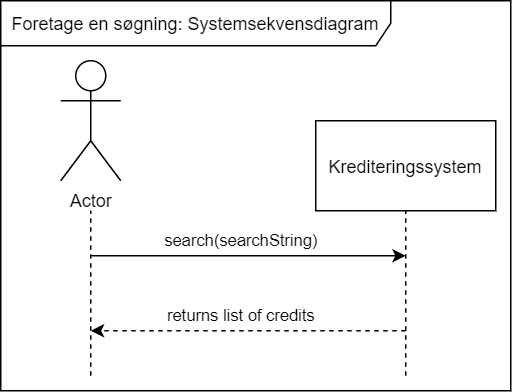
\includegraphics[scale = 0.5]{images/B03SSD.png}
    \caption{Systemsekvensdiagram for search}
    \label{fig:SystemsekvensdiagramSearch}
\end{figure}

Firgur \ref{fig:SystemsekvensdiagramSearch} viser at en aktør, her en bruger, bruger funktionen search på krediteringssystem som derefter returnerer en liste af krediteringer. Ud fra dette diagram blev der opsat en operationskontrakt over hvilket ansvar search operationen har. Denne operationskontrakt ses på tabel \ref{tab:OperationsKontraktB03}

\begin{table}[H]
\centering
\label{tab:1}
    \begin{tabular}{|p{30mm} p{90mm}|} \hline
        \textbf{Kontrakt} &  \\ \hline
        \textbf{Operation} & search(searchString) \\ \hline
        \textbf{Refererer til} & Brugsmønster: Foretag en søgning \\ \hline
        \textbf{Ansvar} & Ansvaret for denne operation er at at modtage en forespørgsel fra en bruger og vise de krediteringer der svarer til forespørgslen, for brugeren hvis:
        \begin{itemize}
            \item Der eksisterer krediteringer der matcher brugerens forespørgsel
            \item Den ønskede kreditering er godkendt af TV 2 moderatorer 
        \end{itemize}
        Den liste som brugeren får vist, vil indeholde en mængde af krediteringer der passer til deres forespørgsel, og kunden kan her vælge en af disse krediteringer, og få yderligere information om den\\ \hline
        \textbf{Prækonditioner} & Datebasen indeholder data\\ \hline
        \textbf{Postkonditioner} & Brugeren får vist en liste af krediteringer som matcher forespørgslen.\\ \hline
    \end{tabular}
        \caption{Operationskontrakt for operationen search}
        \label{tab:OperationsKontraktB03}
\end{table}

Tabel \ref{tab:OperationsKontraktB03} fortæller at ansvaret for search operationen er at finde de krediteringer der matcher brugerens forespørgsel, og returnere dem så de kan ses. Dette kræver at der er data det matcher i databasen som samtidig er godkendt af en TV 2 moderator.
Herefter udarbejdede gruppen et sekvensdiagram for operationer inde i systemet. Først på figur \ref{fig:B03OSDit1} er resultatet for iteration 1, og derefter på figur \ref{fig:OperationsSekvensdiagramSearch} resultatet for iteration 2

\begin{figure}[H]
    %\centering
\centerline{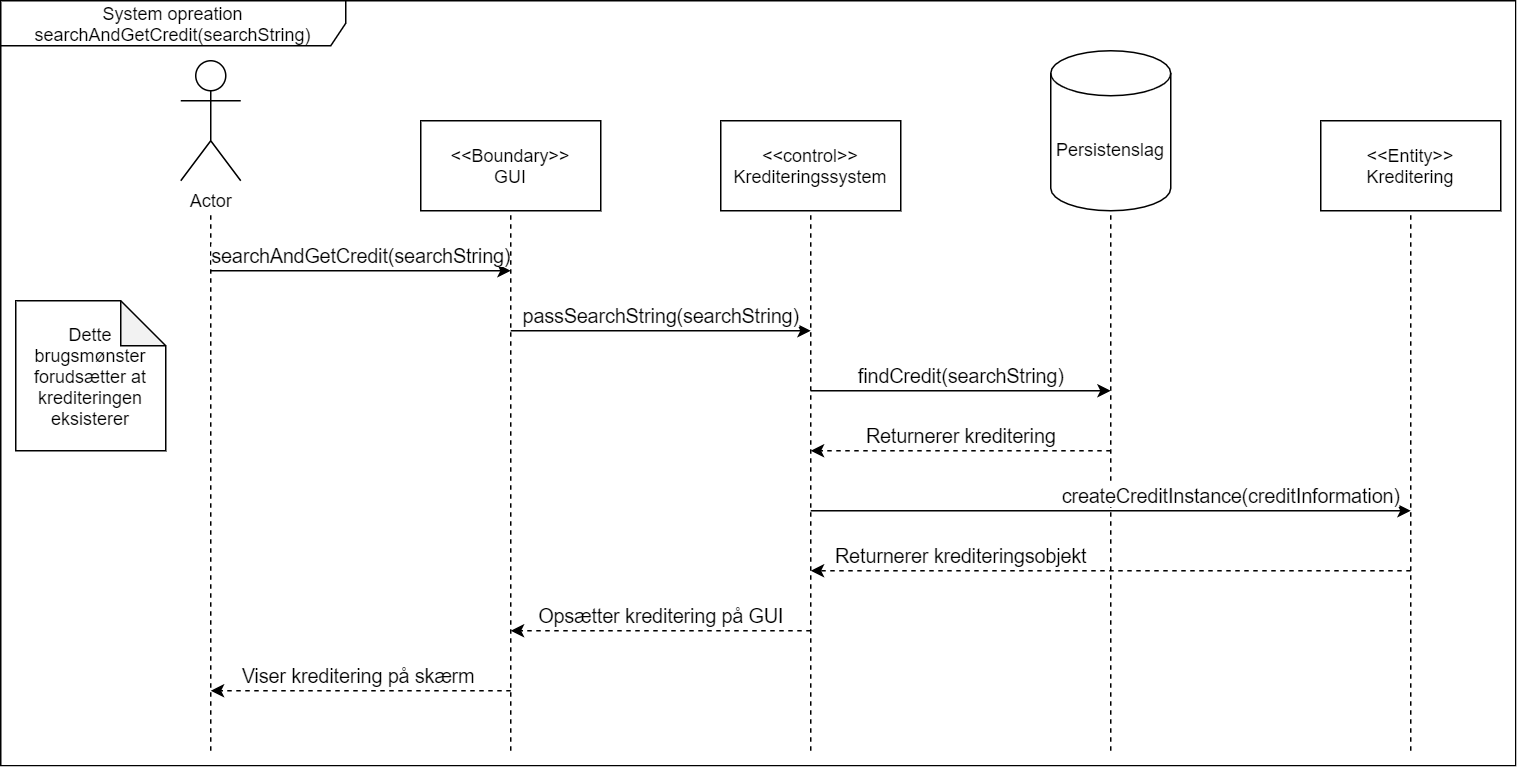
\includegraphics[scale = 0.37]{images/B03OSDit1.png}}
    \caption{Sekvensdiagram for operationer på ved searchAndGetCredit i iteration 1}
    \label{fig:B03OSDit1}
\end{figure}

Iteration 1 var en simpel udgave af programmet og havde ikke vanvittig meget funktionalitet. Figur \ref{fig:B03OSDit1} viser operations sekvensdiagrammet for søgefunktionen searchAndGetCredit der bliver kaldt på GUI delen. GUI'en kalder 



\begin{figure}[H]
    %\centering
\centerline{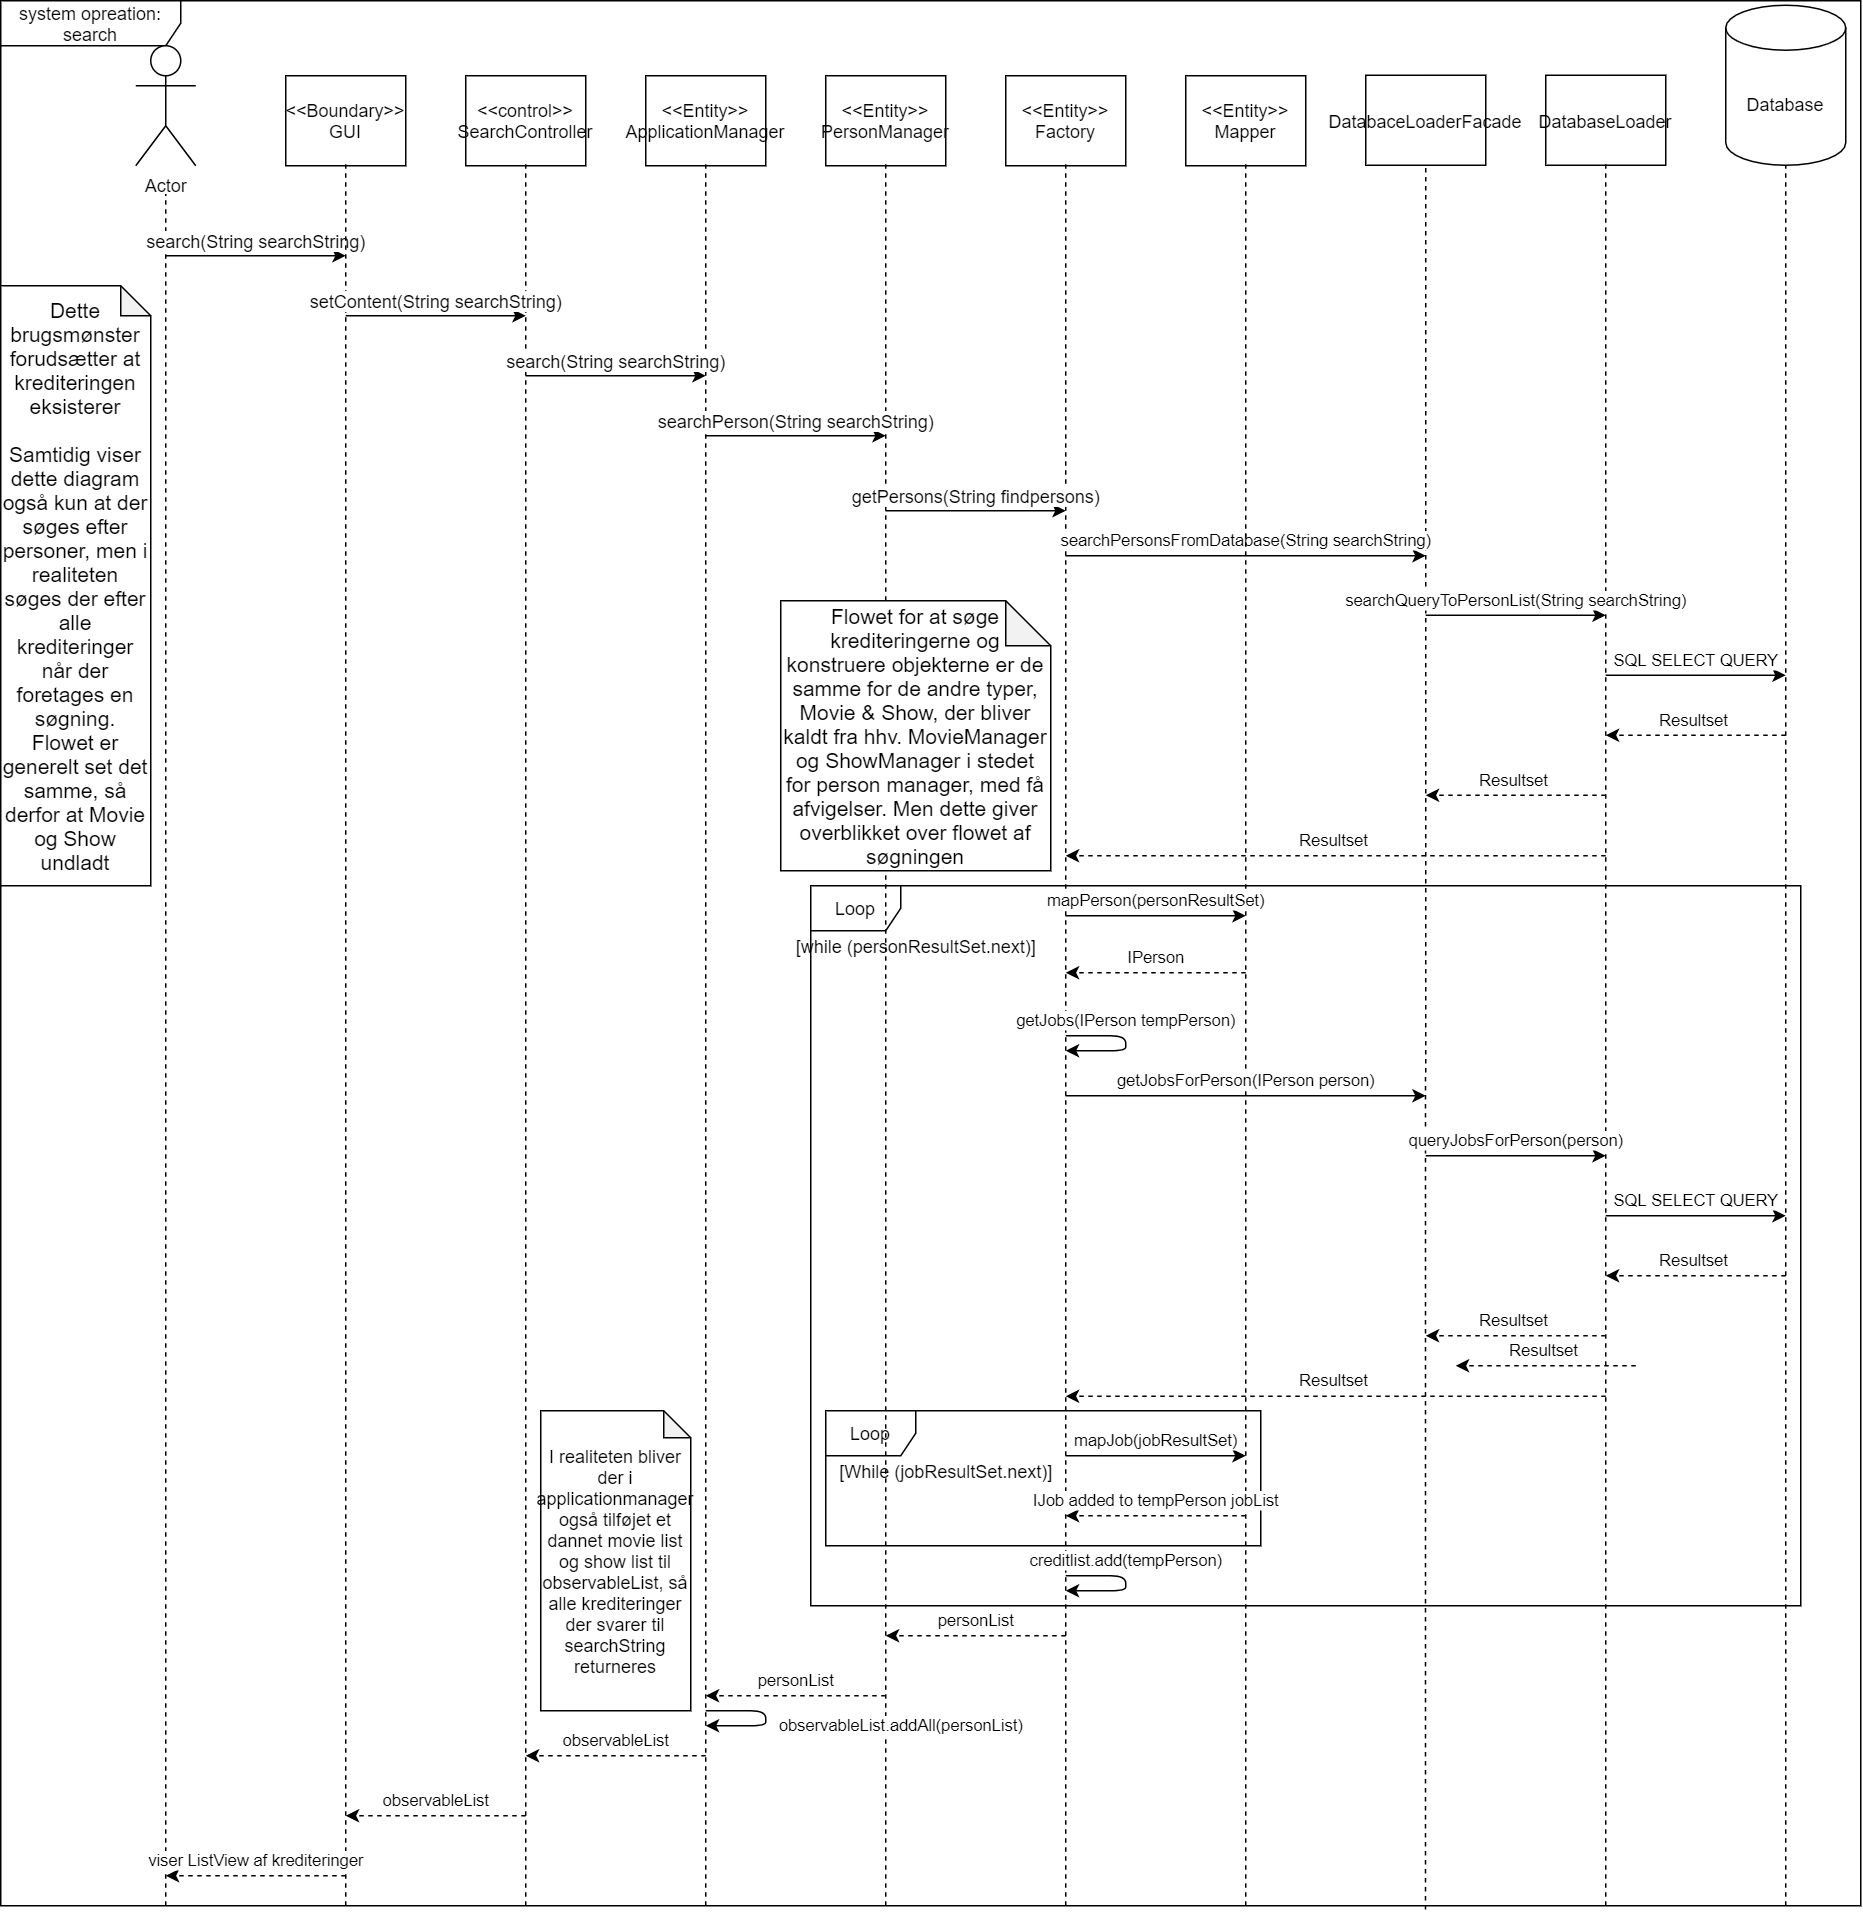
\includegraphics[width = 195mm]{images/B03OSD.png}}
    \caption{Sekvensdiagram for operationer på ved search}
    \label{fig:OperationsSekvensdiagramSearch}
\end{figure}

Operations sekvensdiagrammet på figur \ref{fig:OperationsSekvensdiagramSearch} viser hvilke klasser som systemet går igennem for at lave en søgning. Det starter med at aktøren indtaster sine søgekriterier og trykker søg på GUI'en. Dette kalder funktionen search som tager en string som parameter. Search kalder funktionen setContent på SearchController klassen, som har til ansvar at få en liste fra searchString og vise den liste på GUI. SearchController kalder så funktionen search på application manager, som tager searchString og søger efter de forskellige typer af krediteringer. I dette eksempel vises kun søgningen efter personer, men flowet er det samme for film og serier, og derfor er de ikke medtaget i diagrammet. Application manager kalder searchPerson på PersonManager. PersonManager står for mange af funktonerne på objekter af typen Person. Personmanager kalder derefter getPersons på Factory. Factory er den klasse der står for at afgøre objekter der skal konstrueres og hvor data skal hentes fra. Factory kalder så searchPersonsFromDatabase på DatabaseLoaderFacade og sender igen searchString videre. DatabaseLoaderFacade er den simple indgang til databseLoader, hvor Facaden kalder funktionen searchQueryToPersonList stadig med searchString som parameter. Denne funktion queryer så databasen ved at finde de tupler der minder som søgekriteriet searchString. Databasen returnerer derefter et ResultSet af tupler, som sendes tilbage til Factory gennem DatabaseLoader, og DatabaseLoaderFacade. Her begynder konstruktionen af objekterne. Factory starter et loop, der slutter når der ikke er flere tupler i ResultSettet. For hver tupel, kalder Factory mapPerson på Mapper og sender en tupel som parameter. Metoden mapPersons tager denne tupel, og instantierer et person-objekt som en IPerson. En produktion som denne person har været med på kaldes et job. Factory sender den nyligt instantierede person til databasen (ved samme flow som perons) og får returneret et ResultSet af Jobs der har personens personID. Factory starter igen et loop over alle tupler i ResultSettet og tilføjer et instantieret job til en Arrayliste som sættes til personens jobs variabel. Her er personen konstrueret færdig, og personen tilføjes til et liste af krediteringer, creditList. og loopet kører igen. Når der ikke er flere tupler, returneres creditList, først gennem PersonManager, til ApplicationManger der tilføjer listen med personer til en generel list af Krediteringer. Her vil ApplicationManager så søge efter de nadre typer af krediteringer, film og serier, og tilføje dem til listen også. Når dette er gjort, laves listen om til en ObservableList som returneres til SearchController som sætter et ListView på GUI til at vise denne Observable list, og her får aktøren så vist listen af krediteringer der svarer til deres søgning.